\subsection{Časovače a počítadlá}
\noindent

Ako názov napovedá, časovače sú určené na meranie času. Často ich nazývame aj počítadlá
pretože vo svojom základnom princípe časovače len počítajú počet dokončených periód zdrojových hodín.
Každý časovač má svoj vlastný register, kde je uložená jeho aktuálna hodnota a taktiež každý potrebuje zdroj hodín. V mikrokontroléroch často existuje niekoľko možných zdrojov
hodín a ich výber je možné určiť pomocou prepínača. Niektoré mikrokontroléry umožňujú aj použitie
externých hodín \cite{IntroductionMicrocontrollerTimers}. \par
Fungovanie časovača si najlepšie opíšeme na konkrétnom príklade.
Uvažujme časovač s 16-bitovým registrom a zdrojom hodín s frekvenciou 1 kilohertz. Po každom uplynutí cyklu v hodinách, časovač
zvýši hodnotu uloženú v registri o 1. Dĺžku jedného cyklu časovača je možné vyjadriť vzorcom:

\[Dĺžka\:cyklu =\frac{1}{Frekvencia\:hodín}\]
To znamená že najkratší časový úsek, ktorý je možné pomocou časovača odmeriať sa
rovná dĺžke periódy vstupných hodín. V našom príklade s hodinami s frekvenciou 1 kilohertz je dĺžka periódy nasledovná:
\begin{equation}
    \begin{aligned}
        Dĺžka\:cyklu & = \frac{1}{Frekvencia\:hodín} \\
                     & = \frac{1}{1kHz}              \\
                     & = \frac{1}{ 1000 Hz}          \\
                     & =  0.001\:sekundy
    \end{aligned}
\end{equation}
Dĺžka periódy je 0.001 sekundy. Z toho vyplýva, že časovač je schopný odmerať dĺžku času, ktorý je násobkom 0.001. Ak necháme časovač napočítať do 100, potrvá to 100 krát 0.001 sekundy, čiže 0.1 sekundy \cite{cameraNewbieGuideAVR2015}. Tu treba poznamenať, že v našom príklade počítame s frekvenciou 1kHz, čo je pomerne nízka frekvencia a dnešné mikrokontroléry sú podstatne rýchlejšie. Ako príklad uvedieme mikrokontrolér Arduino Mega2560, ktorý používa frekvenciu 16MHz čo je rádovo viac ako 1kHz \cite{ArduinoMega2560}.
\par Pre reálnejšiu predstavu preto pokračujme v našom príklade s časovačom s frekvenciou 1MHz. Časovač má k dispozícii 16-bitový register. Maximálny počet
možných hodnôt v registri je teda $2^{16}$ (65536, maximálna hodnota je 65365).
Po dosiahnutí maximálnej hodnoty register pretečie a časovač začne počítať znova od 0.
\begin{figure}[!h]
    \centering
    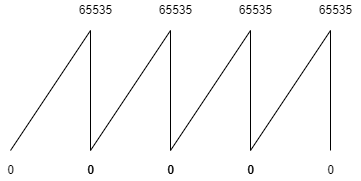
\includegraphics[width=0.70\textwidth]{img/timer.png}
    \caption{Zmena hodnoty v 16 bitovom registri časovača.}
    \label{figure:timer1}
\end{figure}

Pri hodinách s frekvenciou 1MHz časovač dosiahne maximálnu hodnotu registra približne každých 66 milisekúnd a dĺžka jedného cyklu je $\frac{1}{1000000}$ sekundy, čo je 1 mikrosekunda \cite{cameraNewbieGuideAVR2015}.

\subsubsection{Preddelička}

Pri použití 16-bitového registra je 66 milisekúnd najdhlší časový interval, ktorý dokážeme odmeriať pokým register nepretečie a časovač nezačne počítať od 0.
Pre nás ľudí je to veľmi krátky časový úsek. Často chceme dosiahnuť interval, ktorý je dlhší a pre nás badateľný. Príkladom takého intervalu je  napríklad 1 sekunda. Existuje viacero spôsobov ako tento interval dosiahnuť, jedným z nich je použitie preddeličky (v anglickej literatúre sa používa termín prescaler).
\par
Preddelička je súčasťou obvodu časovača, ktorý nám umožňuje preskočiť periódy zdrojových hodín o mocninu 2, čím sa zníži frekvencia, ale zároveň dostaneme dlhší rozsah časovača.
Hodnoty preddeličky bývajú pevne dané a často sú to hodnoty 1, 8, 64, 256 a 1024. Vzorec pre výpočet dĺžky cyklu spolu s preddeličkou je nasledovný:

\begin{equation}
    \begin{aligned}
        Dĺžka\:cyklu & = \frac{1}{\frac{Frekvencia\:hodín}{Preddelička}} \\
                     & = \frac{Preddelička}{Frekvencia\:hodín}           \\
    \end{aligned}
\end{equation}

Pre časovač s frekvenciou 1MHz a hodnotami preddeličky 1, 8, 64, 256 s 1024 môžme zostrojiť nasledujúcu tabuľku:
\begin{table}[!htbp]
    \begin{center}
        \begin{tabular}{|c|c|}
            \hline
            Hodnota preddeličky & Dĺžka cyklu časovača \\
            \hline
            1                   & 1 $\mu s$            \\
            8                   & 8 $\mu s$            \\
            64                  & 64 $\mu s$           \\
            256                 & 256 $\mu s$          \\
            1024                & 1024 $\mu s$         \\
            \hline
        \end{tabular}
        \caption{Dĺžka cyklu 1MHz časovača pri rôznych hodnotách preddeličky}
        \label{table:timerPrescaler}
    \end{center}
\end{table}

Pre dosiahnutie 1 sekundového intervalu potrebujeme poznať aj hodnotu registra
pri ktorej tento interval uplynie. Tú dosataneme použitím nasledujúceho vzorca:

\begin{equation}
    \begin{aligned}
        Hodnota\:registra & = \frac{ \frac{1}{Cieľová\:frekvencia}} { \frac{Preddelička}{Frekvencia\:hodín}} - 1 \\
                          & = (\frac{Frekvencia\:hodín}{Preddelička \times Cieľová\:frekvencia}) - 1             \\
    \end{aligned}
\end{equation}

Časovače AVR TODO!! aktualizujú svoju hodnotu iba pri každom tiknutí vstupných hodín. Je teda potrebný tik aby sa hodnota časovača dostala z maximálnej hodnoty späť na nulu. Preto v znáronenom vzorci
musíme znížiť počet tikov o jeden. \par

Teraz sa vráťme späť k tomu ako dosiahneme interval 1 sekundy. Potrebujeme zistiť či existuje hodnota preddeličky, ktorá poskytne presné oneskorenie 1 Hz. Jeden Hertz je rovný jednému cyklu za sekundu.
Výsledky umiestnime do tabuľky č. \ref{table:timerPrescalerValues}:

\begin{table}[!htbp]
    \begin{center}
        \begin{tabular}{|c|c|}
            \hline
            Hodnota preddeličky & Hodnota registra časovača \\
            \hline
            1                   & 999999                    \\
            8                   & 124999                    \\
            64                  & 15624                     \\
            256                 & 3905,25                   \\
            1024                & 975,5625                  \\
            \hline
        \end{tabular}
        \caption{Potrebná hodnota v registri 1MHz časovača pre dosiahnutie 1 sekundového intervalu}
        \label{table:timerPrescalerValues}
    \end{center}
\end{table}

Pri pohľade na tabuľku môžeme hneď usúdiť, že preddeličky s hodnotou 256 a 1024 niesú vhodné pre dosiahnutie nášho cieľa. Hodnota v registri je vždy celé kladné číslo a preto nemôžme tieto hodnoty použiť. Ďalším kritériom pre výber preddeličky je veľkosť
vypočítanej hodnoty. Náš časovač používa 16-bitový register, ktorého maximálna hodnota je $2^{16} -1$ (65365).
Ostáva nám teda len jedna možnosť preddeličky: a to 64. Preddeličky s hodnotou 1 a 8 vyžadujú hodnotu registra väčšiu ako je schopný uložiť. Suma sumárum, pre dosiahnutie jedno sekundového intervalu pomocou 16 bitového časovača s frekvenciou 1MHz potrebujeme použiť preddeličku s hodnotou 64. 1 sekundu časovač dosiane po napočítaní do 15624. \par
Čo však v prípade ak chceme dosiahnuť dlho trvajúce intervaly? Hodinu, deň, týždeň, mesiac prípadne rok?
V tomto prípade je možné implementovať preddeličku aj softvérovo. Pre jednoduchšie vysvetlenie si riešenie problému ukážeme na príklade. Uvažujme rovnaké parametre časovača: 1MHz frekvencia, 16 bitový register. Chceme dosiahnuť časový interval jednej hodiny. Pomocou vyššie popísanej techniky vytvoríme interval 1 sekundy.
Po každom uplynutí intervalu zvýšime hodnotu nášho počítadlá. 1 hodina je 3600 sekúnd. Teda vieme že pokiaľ naše počítadlo dosiahne hodnotu 3600 ubehla 1 hodina.
Pseudokód danej implementácie by mohol vyzerať nasledovne:
\begin{lstlisting}[
    label={lst:main-c},
    language=c
  ]  
Initialise counter to 0
WHILE forever
    IF timer value IS EQUAL TO 1 sec THEN
        Increment counter
        Reset timer
        IF counter value IS EQUAL TO 3600 THEN
            // 1 HOUR HAS PASSED
            Reset counter
        END IF
    END IF
END WHILE
\end{lstlisting}
Pri takejto implementácii je potrebné dať si pozor aj na najmenšie odchýlky od základného intervalu, ktorý je nastavený pomocou hardvérovej preddeličky. Aj najmenšia odchýlka môže po sčítaní znamenať veľkú nepresnosť v požadovanom konečnom intervale \cite{cameraNewbieGuideAVR2015}.

\subsubsection{Časovače a prerušenia}

\subsubsection{CTC mód}

\subsubsection{PWM mód}